\chapter{Implementation}

Part of this thesis is to implement asynchronous duet benchmark super-harness that takes existing benchmark harness as an input and executes its benchmarks in asynchronous duet style.
This kind of tool should greatly simplify general use of asynchronous duet method.

% Running in docker and reasons for it
To keep a configuration portable and the dependencies minimal we have decided to use the container technology, namely Docker~\cite{merkel2014docker} or Podman~\footnote{\url{https://podman.io/}, July 2022}.
Tool is named \lstinline{duetbench} and it is part of open sourced~\footnote{Apache Licence 2.0} python package \lstinline{duet}~\footnote{\url{https://github.com/TomasDrozdik/asynchronous-duet}, July 2022} that also implements other complementary tools~\cref{sec:result_parsing}.
Source code is available as attachment to this thesis~\xxx{ref} and it has documentation in form of GitHub wiki~\cite{wiki}.

% Docker -> different environment -> support for both sequential and synchronous duet runs
Since one of the goals of this thesis is to compare asynchronous duet with synchronous and sequential method usage of containers makes direct comparison with~\citet{bulej2020duet} unreasonable.
Therefore \lstinline{duetbench} supports all three benchmarking methods in containerized environment.

\section{Architecture}

\Cref{fig:duetbench_sequence} depicts architecture of \lstinline{duetbench} script.
\lstinline{duetbench} is a process on host machine that spawns subprocesses that run containers --- one for each version A/B.
Since initialization of a container might take longer \lstinline{duetbench} waits for both containers to start and then uses \lstinline{docker exec}~\footnote{\lstinline{docker exec} reference \url{https://docs.docker.com/engine/reference/commandline/exec/}, July 2022} to run the command that executes the benchmark harness loop from~\cref{alg:harness}.
Then once both benchmarks finish, copy raw result of those benchmarks from respective containers and store them in some fixed format to preserve information about particular run.
Afterwards stop and cleanup both containers.

\begin{figure}
	\centering
	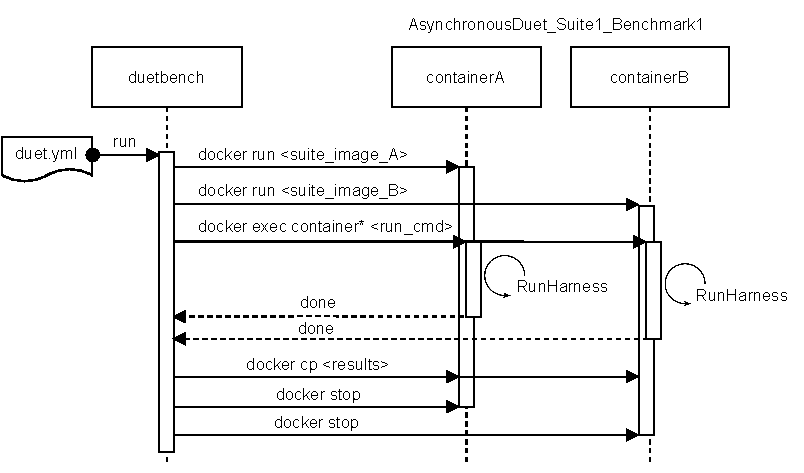
\includegraphics[width=\linewidth]{./figures/duetbench-sequence.drawio.pdf}
	\caption{
        UML sequence diagram of how \lstinline{duetbench} executes a single A/B asynchronous duet benchmark.
        Note that the docker commands are simplyfied for brevity.
        All the parameters in angled brackets are specified in configuration file \lstinline{duet.yml}~\cref{sec:configuration}.
	}
	\label{fig:duetbench_sequence}
\end{figure}

If there are more benchmarks to execute pick next one and do the same process.
In case of the sequential method, the process is very much the same just omit the second container entirely and run them separately.

\subsection{Synchronized duet in containerized environment}

In case of the synchronized duet, benchmark harness needs to be modified as in~\citet{bulej2020duet}.
Additionally,~\citet{bulej2020duet} synchronize the iterations using shared memory barrier placed in \lstinline{/dev/shm} before benchmarks are started.
Then each benchmark invocation gets path to this shared barrier file and their harness blocks on this barrier before each iteration.
To facilitate similar behavior between containers \lstinline{duetbench} starts the dockers with mounted volumes \lstinline{-v /dev/shm:/dev/shm} and shared inter process communication namespace \lstinline{--ipc host}~\footnote{\lstinline{docker run} reference \url{https://docs.docker.com/engine/reference/run/}, July 2022}.
Last but not least, something has to create this shared memory barrier and clean it up afterwards.

Barrier is made with \lstinline{pthread_barrier_init}~\footnote{\lstinline{man 3 pthread_barrier_init}}, however this call is not available on all Unixes for example macOS~\footnote{macOS Monterey Version 12.3.1}.
Instead, \lstinline{duetbench} creates these barriers from one of the containers, since both have mounted the same volume \lstinline{/dev/shm}.
Advantage of such approach is that docker containers access to \lstinline{pthread_barrier_init} even though underlying host might not~\footnote{Since Docker on both macOS and Windows still runs Linux VM underneath docker containers \url{https://www.docker.com/blog/the-magic-behind-the-scenes-of-docker-desktop/}, July 2022}.

\section{Configuration}
\label{sec:configuration}

\Cref{lst:config} shows section of \lstinline{duetbench} YAML configuration file that describes an A/B asynchronous duet and sequential run.
Goal of the design was to make configuration generic and simple to use so that many harnesses and benchmark suites can be adapted to use with \lstinline{duetbench}.
Full documentation of the \lstinline{duetbench} configuration including description of how to run synchronized duets not present in the~\cref{lst:config} is on the wiki~\cite{wiki}.

Freedom in run command allows for tweaking of the harness to better suite asynchronous duet, for example some harnesses support skips of validation or various garbage collector options.
Detailed configuration of experiments is in~\cref{sec:benchmark_configuration}.

\begin{listing}
    \begin{lstlisting}
avrora:
  image: dacapo
  duet_repetitions: 2
  sequential_repetitions: 2
  schedule: randomized_interleaving_trials
  A:
    run: java -jar dacapo-A.jar -n 50 -o results.csv avrora
  B:
    run: java -jar dacapo-B.jar -n 50 -o results.csv avrora
  results:
    - results.csv
    \end{lstlisting}
    \caption{
        Example part of YAML configuration file for \lstinline{duetbench} that runs \lstinline{avrora} benchmark from the Dacapo suite.
        In this case both A and B versions are packaged in single container image as Java JAR archives.
        Run command specifies how to invoke the dacapo harness --- 50 iterations, results in \lstinline{results.csv} and run only \lstinline{avrora} benchmark.
        All the result files or directories need to specified in \lstinline{results} array field.
        Note correspondence between user input fields from this configuration and parameters in angled brackets from~\cref{fig:duetbench_sequence}.
        Furthermore, user can specify number of repetitions for both asynchronous duet and sequential measurements, as well as scheduling strategy for those runs.
    }
    \label{lst:config}
\end{listing}

\subsection{Run scheduling}

As \lstinline{duetbench} is a harness that runs other harnesses this is some terminology used in the \lstinline{duet} package:

\begin{description}
    \item[Pair] $p$ is version of tested software $p \in P | P = \{A, B\}$
    \item[Type] $t$ is the measurement method type
        $t \in T | T = \{sequential, synchronous\_duet, asynchronous\_duet\}$
    \item[Benchmark] $b$ is some benchmark from particular benchmark suite
        $b \in B | B = \{(suite, benchmark) | suite \in Suites \& benchmark \in suite\}$
    \item[Run] $r$ is invocation of a benchmark $b \in B$ with measurement type $t \in T$ on pair $p \in P$.
        Formally $r \subset B \times T \times P$. It is unit that \lstinline{duetbench} works with and can repeat multiple times. In some papers this is referred to as trial~\cite{laaber2019software}.
    \item[Iteration] $i$ is a single iteration of some run $r \in R$. Duration of an iteration is a data point of an experiment. A run typically runs fixed number of iterations of some benchmark, refer to experiment setup in~\cref{sec:experiment_setup} for more details.
\end{description}

Scheduling of runs is done in RMIT~\cite{abedi2017conducting}, however in this context we interleave also different types of measurement of different benchmarks.

\section{Result parsing}
\label{sec:result_parsing}

Once a run finishes, results are copied in their raw format to a dedicated result directory on the host machine.
Results are then processed to some common format for further analysis.
For this purpose \lstinline{duet} package has \lstinline{duetprocess} script~\cite{wiki}.
It takes an output directory of \lstinline{duetbench} and produces single results file in CSV format.

Minimal schema of result data point looks like this:
\begin{itemize}
    \item Directly parsed by \lstinline{duetprocess}:
        \begin{itemize}
            \item suite
            \item benchmark
            \item run: repetetion id, not necessarily run in order
            \item pair
            \item pair order: which pair was started first
            \item iteration
            \item artifacts: \lstinline{duetbench} provides and option to run some additional commands such as \lstinline{lscpu} or \lstinline{cat /proc/meminfo} to obtain information about host environment
        \end{itemize}
    \item Specific per benchmark suite parsers:
        \begin{itemize}
            \item iteration start timestamp (ns)
            \item iteration end timestamp (ns)
        \end{itemize}
\end{itemize}

Since different benchmarks suites have wildely different results formats users have to write parser plugin --- python function.
Parser has to obtains iteration start and end timestamps from benchmark results. 
Additionally, since users need to write parser for given benchmark suite, they might add any sort of data that benchmark produces in addition to above mentioned data.

Some benchmarks suites don't track absolute timestamps of iterations and thus need some modification.
However, without absolute timestamps one could not assert whether iterations actually overlap and address \emph{RQ2}.
